\documentclass{article}%
\usepackage[T1]{fontenc}%
\usepackage[utf8]{inputenc}%
\usepackage{lmodern}%
\usepackage{textcomp}%
\usepackage{lastpage}%
\usepackage{authblk}%
\usepackage{graphicx}%
%
\title{miR{-}221 Promotes Tumorigenesis in Human Triple Negative Breast Cancer Cells}%
\author{Joanne Jackson}%
\affil{Instituto de Biologa Molecular y Celular de Plantas, Universidad Politcnica de Valencia{-}C.S.I.C, Ciudad Politcnica de la Innovacin, Valencia, Spain}%
\date{01{-}01{-}2011}%
%
\begin{document}%
\normalsize%
\maketitle%
\section{Abstract}%
\label{sec:Abstract}%
CHENNAI {-} India {-} CCL2 has now been found to disrupt the entire cell cycle and attack all normal macrophages.\newline%
The cells of human monocytes which produce CCL2 are a major source of the cancer process in humans. It is thought that the CCL2 mutation has been identified in humans by Indian scientists and a free radical toxin has been introduced. It appears that all stem cells and all normal epidermal growth factor receptor and immune mediators in mouse and human monocytes are switched off. If left unchecked, this blockage to the original CYC2 and CCR2 is brought on by the CCL2 mutations.\newline%
To deal with the power of the leak the CCL2 can simply be divided into three arms: first, an attempt at stimulating the release of CCL2 from the cells, then an attempt at provoking death of the cell through the bodys fight back against the attack of the CCL2 cell and finally, an attempt to increase the production of cancer related proteins.\newline%
The strategy used is to convert the actin or a precursor made by all cultured cells into CCL2 on an enriched scaffold. The specialized ion channel  CGRP is considered the most critical. The transformed phase complex is then given high degree of functionality and leads to increase in its transfer to the whole cell cycle. This process of anisotopic reflowering reveals new targeted ways of conducting the process and is regulated by target factor CGRP.\newline%
Treatment of human monocytes is beginning to be successful and should decrease the immune response required to combat the cancer. CCR2 needs to be removed by CQS (CQRF) signaling. Toxins (lesions of cells) are also required for the uncontrolled release of CCL2. This distantly related pharmacological process sends out a strong signal over the cell membrane which anisotopic reflowering destroys. This will therefore prove a useful tool for the treatment of CCL2.

%
\subsection{Image Analysis}%
\label{subsec:ImageAnalysis}%


\begin{figure}[h!]%
\centering%
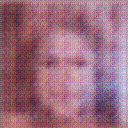
\includegraphics[width=150px]{500_fake_images/samples_5_25.png}%
\caption{A Black And White Photo Of A Black And White Cat}%
\end{figure}

%
\end{document}